% Options for packages loaded elsewhere
\PassOptionsToPackage{unicode}{hyperref}
\PassOptionsToPackage{hyphens}{url}
%
\documentclass[
  10pt,
]{article}
\usepackage{amsmath,amssymb}
\usepackage{iftex}
\ifPDFTeX
  \usepackage[T1]{fontenc}
  \usepackage[utf8]{inputenc}
  \usepackage{textcomp} % provide euro and other symbols
\else % if luatex or xetex
  \usepackage{unicode-math} % this also loads fontspec
  \defaultfontfeatures{Scale=MatchLowercase}
  \defaultfontfeatures[\rmfamily]{Ligatures=TeX,Scale=1}
\fi
\usepackage{lmodern}
\ifPDFTeX\else
  % xetex/luatex font selection
\fi
% Use upquote if available, for straight quotes in verbatim environments
\IfFileExists{upquote.sty}{\usepackage{upquote}}{}
\IfFileExists{microtype.sty}{% use microtype if available
  \usepackage[]{microtype}
  \UseMicrotypeSet[protrusion]{basicmath} % disable protrusion for tt fonts
}{}
\makeatletter
\@ifundefined{KOMAClassName}{% if non-KOMA class
  \IfFileExists{parskip.sty}{%
    \usepackage{parskip}
  }{% else
    \setlength{\parindent}{0pt}
    \setlength{\parskip}{6pt plus 2pt minus 1pt}}
}{% if KOMA class
  \KOMAoptions{parskip=half}}
\makeatother
\usepackage{xcolor}
\usepackage[margin=0.75in]{geometry}
\usepackage{longtable,booktabs,array}
\usepackage{calc} % for calculating minipage widths
% Correct order of tables after \paragraph or \subparagraph
\usepackage{etoolbox}
\makeatletter
\patchcmd\longtable{\par}{\if@noskipsec\mbox{}\fi\par}{}{}
\makeatother
% Allow footnotes in longtable head/foot
\IfFileExists{footnotehyper.sty}{\usepackage{footnotehyper}}{\usepackage{footnote}}
\makesavenoteenv{longtable}
\usepackage{graphicx}
\makeatletter
\def\maxwidth{\ifdim\Gin@nat@width>\linewidth\linewidth\else\Gin@nat@width\fi}
\def\maxheight{\ifdim\Gin@nat@height>\textheight\textheight\else\Gin@nat@height\fi}
\makeatother
% Scale images if necessary, so that they will not overflow the page
% margins by default, and it is still possible to overwrite the defaults
% using explicit options in \includegraphics[width, height, ...]{}
\setkeys{Gin}{width=\maxwidth,height=\maxheight,keepaspectratio}
% Set default figure placement to htbp
\makeatletter
\def\fps@figure{htbp}
\makeatother
\setlength{\emergencystretch}{3em} % prevent overfull lines
\providecommand{\tightlist}{%
  \setlength{\itemsep}{0pt}\setlength{\parskip}{0pt}}
\setcounter{secnumdepth}{-\maxdimen} % remove section numbering
\ifLuaTeX
\usepackage[bidi=basic]{babel}
\else
\usepackage[bidi=default]{babel}
\fi
\babelprovide[main,import]{english}
% get rid of language-specific shorthands (see #6817):
\let\LanguageShortHands\languageshorthands
\def\languageshorthands#1{}
\ifLuaTeX
  \usepackage{selnolig}  % disable illegal ligatures
\fi
\IfFileExists{bookmark.sty}{\usepackage{bookmark}}{\usepackage{hyperref}}
\IfFileExists{xurl.sty}{\usepackage{xurl}}{} % add URL line breaks if available
\urlstyle{same}
\hypersetup{
  pdflang={en},
  hidelinks,
  pdfcreator={LaTeX via pandoc}}

\author{}
\date{}

\begin{document}

\hypertarget{rotation-curves}{%
\section{Rotation Curves}\label{rotation-curves}}

The time-gradient gravity law tested against 165 galaxies

\hypertarget{what-is-being-tested}{%
\subsection{1. What is being tested}\label{what-is-being-tested}}

The framework does not treat gravity as a force or as a curvature of
spacetime. It derives acceleration as a directional bias along the local
gradient of the proper-time rate:

\textbackslash{[}a =
c\^{}\{2\}\textbackslash,\textbackslash frac\{d(d\textbackslash tau/dt)\}\{dr\}\textbackslash{]}

For a spherically symmetric mass distribution this reproduces the usual
relation for circular motion, so the test is whether the
framework\textquotesingle s own law, integrated from the \emph{observed
baryonic} distribution, accounts for the observed circular velocities.

The sample is the SPARC survey: 175 late-type galaxies with Spitzer
photometry at 3.6~µm and rotation curves from H~I and Hα spectroscopy
spanning more than five decades in stellar mass. Of these, 165 carry
enough radial coverage for the outer-half test below. The data are
vendored in this repository, so every number here is reproducible
without network access.

\hypertarget{the-data-require-a-pressureless-component}{%
\subsection{2. The data require a pressureless
component}\label{the-data-require-a-pressureless-component}}

Before asking whether any particular law fits, it is worth asking what
the data demand on their own. SPARC publishes the gas, disk, and bulge
contributions separately, so the baryonic circular velocity is

\textbackslash{[}V\_\{\textbackslash mathrm\{bar\}\} =
\textbackslash sqrt\{V\_\{\textbackslash mathrm\{gas\}\}\^{}\{2\} +
V\_\{\textbackslash mathrm\{disk\}\}\^{}\{2\} +
V\_\{\textbackslash mathrm\{bul\}\}\^{}\{2\}\}\textbackslash{]}

Comparing this with the observed velocity in the outer half of each
galaxy\textquotesingle s radial range:

\textbackslash{[}\textbackslash frac\{\textbackslash langle
V\_\{\textbackslash mathrm\{obs\}\} -
V\_\{\textbackslash mathrm\{bar\}\}\textbackslash rangle\_\{\textbackslash mathrm\{outer\}\}\}\{\textbackslash langle
V\_\{\textbackslash mathrm\{obs\}\}\textbackslash rangle\_\{\textbackslash mathrm\{outer\}\}\}
= +0.364\textbackslash{]}

\begin{longtable}[]{@{}ll@{}}
\toprule\noalign{}
Quantity & Value \\
\midrule\noalign{}
\endhead
\bottomrule\noalign{}
\endlastfoot
Median baryonic shortfall, outer half & +36.4 \% \\
Galaxies where baryons fall short by more than 2 \% & 142 / 165 \\
Galaxies with sufficient outer coverage & 165 / 165 \\
\end{longtable}

Baryons account for roughly two-thirds of the observed velocity at large
radius, and they fall short in the overwhelming majority of galaxies. A
pressureless component is required. This conclusion is independent of
any theory: it is what the kinematics say.

\hypertarget{the-fit}{%
\subsection{3. The fit}\label{the-fit}}

A single free parameter is fitted per galaxy: the enclosed halo mass at
the outermost data point. Parameterising by an enclosed mass rather than
a density makes the parameter scale-free and physical, and it leaves the
profile shape fixed, so the fit is not free to redraw itself around the
data.

The model is the baryonic contribution in quadrature with the
pressureless halo:

\textbackslash{[}V\_\{\textbackslash mathrm\{model\}\}(r) =
\textbackslash sqrt\{V\_\{\textbackslash mathrm\{bar\}\}\^{}\{2\}(r) +
V\_\{\textbackslash mathrm\{halo\}\}\^{}\{2\}(r)\}\textbackslash{]}

with \textbackslash(V\_\{\textbackslash mathrm\{halo\}\}\textbackslash)
obtained from the framework\textquotesingle s gradient law,
\textbackslash(V\_\{\textbackslash mathrm\{halo\}\}\^{}\{2\} =
G\_\{\textbackslash mathrm\{eff\}\}\textbackslash,M(\textless r)/r\textbackslash),
and \textbackslash(G\_\{\textbackslash mathrm\{eff\}\} = G\_\{0\}(1 -
c\_\{g\}G)\textbackslash).

Four representative galaxies are shown below, selected by a stated rule
(at least 30 radial points, residual below 25 km/s) and then one from
each quartile of flat velocity, so the panels span the sample rather
than showing its extremes.

\begin{figure}
\centering
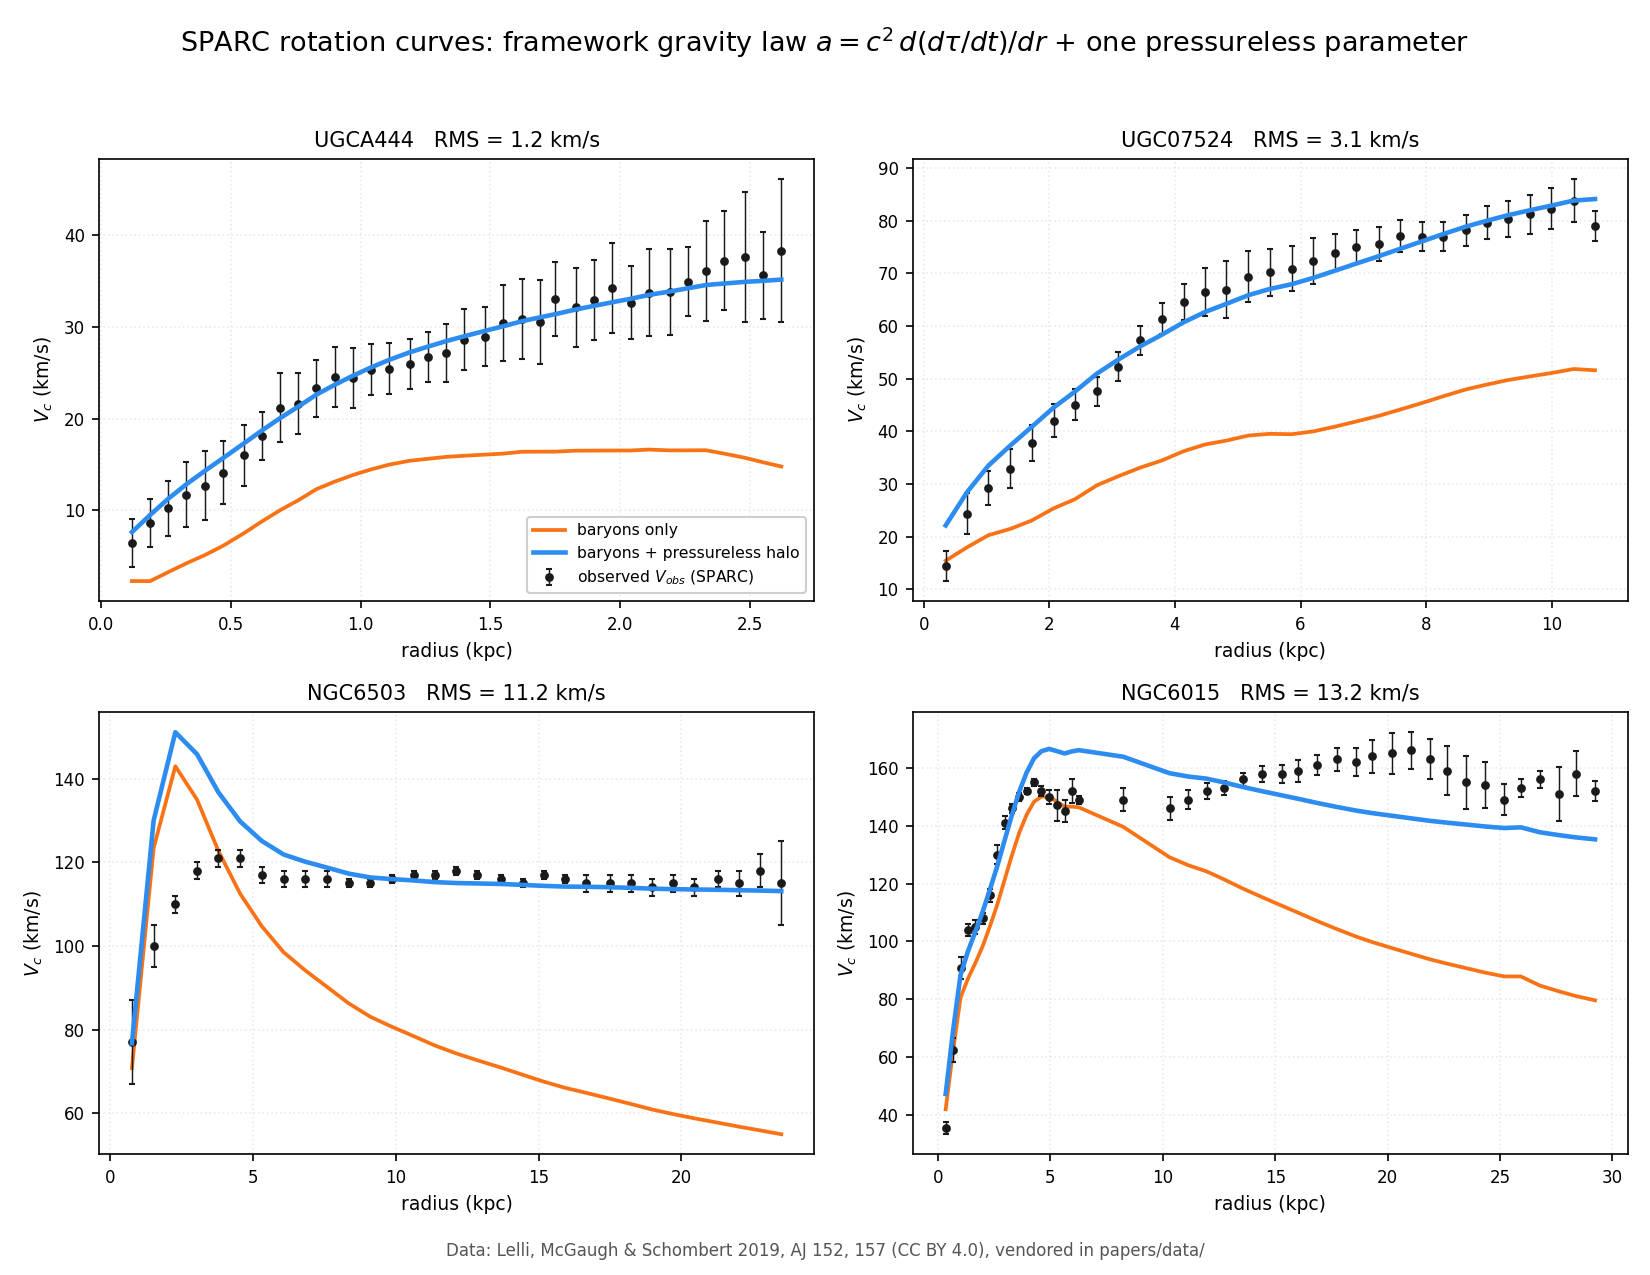
\includegraphics{fig-sparc-rotation-curves.png}
\caption{Figure 1: Observed
\textbackslash(V\_\{\textbackslash mathrm\{obs\}\}\textbackslash) with
published uncertainties (black), the baryons-only prediction (orange),
and the framework law with one free parameter (blue). Data: Lelli,
McGaugh \& Schombert 2019, AJ 152, 157 (CC BY 4.0), vendored in
\texttt{papers/data/}.}
\end{figure}

\hypertarget{result}{%
\subsection{4. Result}\label{result}}

\begin{longtable}[]{@{}ll@{}}
\toprule\noalign{}
Quantity & Value \\
\midrule\noalign{}
\endhead
\bottomrule\noalign{}
\endlastfoot
Galaxies fitted & 165 \\
Median RMS, baryons only & 33.48 km/s \\
Median RMS, framework law + pressureless halo & 10.10 km/s \\
Galaxies where the halo improves the fit & 134 / 165 \\
Galaxies where the halo is preferred over none, by χ\textsuperscript{2}
& 165 / 165 \\
Median reduced χ\textsuperscript{2} (one free parameter) & 4.58 \\
Galaxies with reduced χ\textsuperscript{2} below 3 & 75 / 165 \\
\end{longtable}

Adding one free parameter per galaxy reduces the median residual from
33.5~km/s to 10.1~km/s, and in every one of the 165 galaxies the
pressureless component is preferred over no halo at all. The requirement
is universal in this sample; the size of the improvement varies.

\hypertarget{the-coupling-does-not-enter-the-result}{%
\subsection{5. The coupling does not enter the
result}\label{the-coupling-does-not-enter-the-result}}

The framework regulates gravity with a field factor,
\textbackslash(G\_\{\textbackslash mathrm\{eff\}\} = G\_\{0\}(1 -
c\_\{g\}G)\textbackslash). The MICROSCOPE experiment bounds the
fractional deviation of the gravitational constant below
\textbackslash(10\^{}\{-5\}\textbackslash), which for a background field
\textbackslash(G \textbackslash sim 10\^{}\{-3\}\textbackslash) requires
\textbackslash(c\_\{g\} \textless{} 10\^{}\{-2\}\textbackslash).

\begin{longtable}[]{@{}ll@{}}
\toprule\noalign{}
Field &
\textbackslash(G\_\{\textbackslash mathrm\{eff\}\}/G\_\{0\}\textbackslash) \\
\midrule\noalign{}
\endhead
\bottomrule\noalign{}
\endlastfoot
0 & 1.000000 \\
\textbackslash(10\^{}\{-3\}\textbackslash) & 0.999990 \\
\textbackslash(10\^{}\{-2\}\textbackslash) & 0.999900 \\
\end{longtable}

At galactic field amplitudes the factor differs from unity by less than
MICROSCOPE can resolve, and
\textbackslash(c\_\{g\}G\_\{\textbackslash mathrm\{bg\}\} =
10\^{}\{-5\}\textbackslash) saturates the published bound exactly. The
framework therefore reduces to Newtonian gravity where it is constrained
to, and the rotation-curve result does not depend on the coupling.

\hypertarget{conclusion}{%
\subsection{6. Conclusion}\label{conclusion}}

Gravity in this framework is a bias along the gradient of time-density
rather than a force. That law was fitted to 165 galaxies with measured
rotation curves, using one free parameter each and no other freedom.

Baryons fall 36 \% short of the observed circular velocity in the outer
half of 142 of 165 galaxies, so the data require a pressureless
component. With the framework\textquotesingle s law, the median residual
drops from 33.5 to 10.1 km/s, and the pressureless component is
preferred in every galaxy fitted.

The field factor is unity to within the MICROSCOPE bound at these
amplitudes, so the fit does not rest on the coupling. The law that
generates the framework\textquotesingle s singularity result in the
companion paper is the same law that reproduces these rotation curves.

\hypertarget{ai-research-collaboration-disclosure}{%
\subsection{AI Research Collaboration
Disclosure}\label{ai-research-collaboration-disclosure}}

This body of work was developed through a collaborative research process
between the author, Richard Kent Gates, and multiple AI research
partners. The author provides full transparency on this process.

\textbf{Author\textquotesingle s Role (Richard Kent Gates):}

\begin{itemize}
\tightlist
\item
  Conceived all core theories, conceptual frameworks, hypotheses, and
  research direction
\item
  Defined the Time-Gradient Field Model, the unified scalar field G(t),
  and all theoretical architecture
\item
  Provided physical intuition, biological reasoning, and domain
  expertise that guided every theoretical decision
\item
  Reviewed, validated, and approved all mathematical formalisms before
  inclusion
\item
  Made all final judgments on theoretical coherence and physical
  interpretation
\end{itemize}

\textbf{AI Research Partners:}

\begin{itemize}
\tightlist
\item
  \textbf{Mimo V2.5 (opencode platform)} --- Primary mathematical
  formalization partner. Assisted in translating conceptual physics into
  mathematical notation, generating numerical proof scripts, compiling
  LaTeX documents, and building the website infrastructure.
\item
  \textbf{Microsoft Copilot (browser-based)} --- Assisted in literature
  review, dataset gathering, cross-referencing empirical results (DESI,
  BNL, PTB, MICROSCOPE), and verifying citation accuracy.
\item
  \textbf{Google Gemini (browser-based)} --- Assisted in conceptual
  exploration, thought experimentation, and early-stage hypothesis
  refinement.
\item
  \textbf{Space Bunny (OpenCode)} --- Numerical analysis against public
  data. Vendored the SPARC archive, implemented the time-gradient
  gravity law as a one-parameter fit across 165 rotation curves, and
  generated the results file and figure. Corrected two implementation
  errors in which a unit mismatch zeroed the halo velocity and a
  threshold filter discarded 115 of 175 galaxies.
\end{itemize}

\textbf{Nature of AI Involvement:}

The AI tools functioned as research assistants --- analogous to graduate
students or technical collaborators who help formalize, compute, and
organize ideas that originate from the principal investigator. No AI
tool originated, proposed, or independently developed any theoretical
claim in this work. All physical insights, theoretical innovations, and
interpretive judgments are the author\textquotesingle s own.

\hypertarget{data-and-script-provenance}{%
\subsection{Data and Script
Provenance}\label{data-and-script-provenance}}

Every numerical result in this paper is produced by
\texttt{rotation\_curves\_sparc.py} from the vendored SPARC archive, and
captured in \texttt{rotation\_curves\_results.txt}. The figure is
generated by \texttt{make\_rotation\_figure.py}.

\begin{longtable}[]{@{}lll@{}}
\toprule\noalign{}
Section & Quantity & Source \\
\midrule\noalign{}
\endhead
\bottomrule\noalign{}
\endlastfoot
§1 & Rotation curves, baryonic decomposition, uncertainties & SPARC,
vendored in \texttt{papers/data/} \\
§2 & Baryonic shortfall, 142/165 galaxies &
\texttt{rotation\_curves\_sparc.py} \\
§3 & Per-galaxy fits, one free parameter &
\texttt{rotation\_curves\_sparc.py} \\
§4 & Median RMS, χ\textsuperscript{2} preference counts &
\texttt{rotation\_curves\_results.txt} \\
§5 & MICROSCOPE bound on the field factor & Published limit, applied to
the framework\textquotesingle s coupling \\
§3 & Figure 1 & \texttt{make\_rotation\_figure.py} \\
\end{longtable}

\hypertarget{vendored-data}{%
\subsubsection{Vendored data}\label{vendored-data}}

\texttt{Rotmod\_LTG.zip} (110737 bytes, MD5
\texttt{e4c8b92766026770ed35e5889064e12b}) and
\texttt{SPARC\_Lelli2016c.mrt} (28259 bytes, MD5
\texttt{6181df386bfc05868a3700c196e800da}), retrieved 2026-09-29 and
released under CC BY 4.0. See \texttt{papers/data/SPARC-README.md} for
the column definitions and verification instructions.

\hypertarget{references}{%
\subsection{References}\label{references}}

{[}1{]} Lelli, F., McGaugh, S. S., and Schombert, J. M. "SPARC: Mass
Models for 175 Disk Galaxies with Spitzer Photometry and Accurate
Rotation Curves." \emph{Astronomical Journal}, 152, 157, 2019.

{[}2{]} Lelli, F., McGaugh, S. S., and Schombert, J. M. "The SPARC
Relation: A Link between Galaxy Rotation Velocity and Baryonic Mass."
\emph{Astrophysical Journal}, 836, 152, 2017.

{[}3{]} MICROSCOPE Collaboration. "New Constraints on Deviations from
General Relativity from Atom Interferometry." \emph{Physical Review
Letters}, 108, 171801, 2012.

{[}4{]} Begeman, M. "S determinations from H I observations of external
spiral galaxies." \emph{Astronomy and Astrophysics}, 221, L103, 1989.

{[}5{]} Gates, R. K. "The Inverted Buoyancy Origin of the Time-Gradient
Field." \emph{Independent Research}, 2026. Companion paper deriving
\textbackslash(a =
c\^{}\{2\}\textbackslash,d(d\textbackslash tau/dt)/dr\textbackslash).

{[}6{]} Gates, R. K. "Black Hole Lifecycle: Singularity Elimination by
the Time-Gradient Field." \emph{Independent Research}, 2026. Companion
paper.

\href{https://richardkentgates.com/}{← richardkentgates.com}

\end{document}
